\section{Background and Motivation}\label{sec:background}

\subsection{PFC deadlock problem}\label{subsec:pfcdeadlock}



\textbf{Priority-based Flow Control (PFC)}: The deployment of RDMA over Ethernet requires PFC  to provide a lossless L2 network. PFC is a mechanism for ensuring zero packet loss under congestion in data center bridging (DCB) networks. PFC allows an overwhelmed network device to send a PAUSE frame to its immediate upstream device, which halts the transmission of the sender for a specified period of time.  

PFC works in a per ingress queue fashion. When PFC is enabled, the switch will maintain a counter to track the virtual queue length of each ingress queue. Once the queue length exceeds a pre-configured PFC threshold, a PAUSE frame will be generated.



\textbf{PFC deadlock problem:} The using of PFC can cause deadlock problem. In Fig.~\ref{fig:deadlock_case}, we use a simple example to show how  deadlock can be created when there is a cyclic buffer dependency among a set of switch buffers.

\begin{figure}[t]
	\centering
	
	\subfloat[short for lof][Topology and flows.] {
		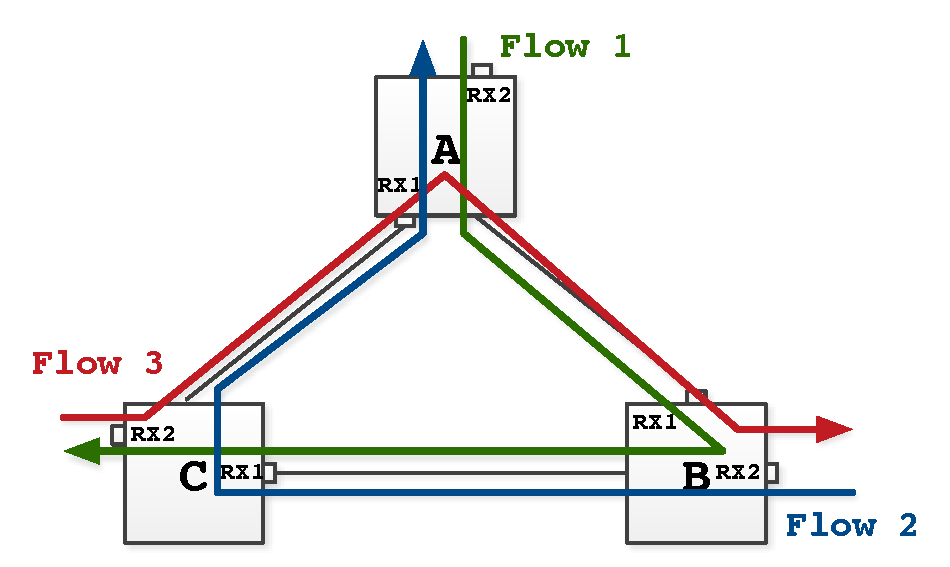
\includegraphics[width=0.3\textwidth] {figs/case1_topo}
	}
	\subfloat[short for lof][Buffer dependency graph.]{
		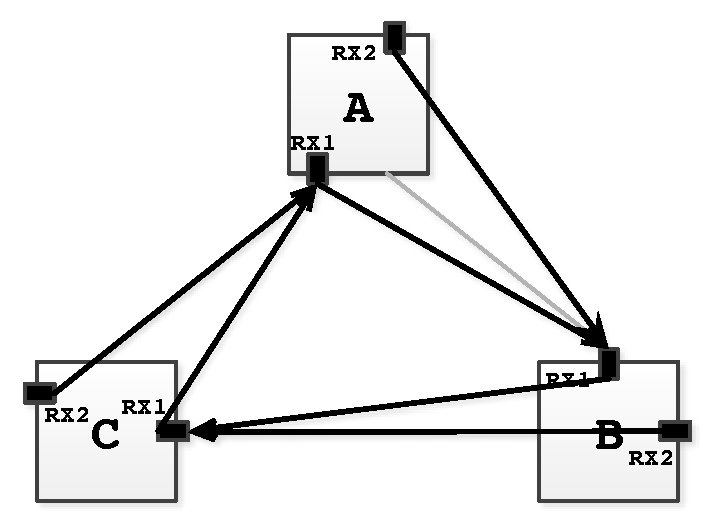
\includegraphics[width=0.2\textwidth] {figs/case1_dependency}
	}
	
	\caption{Flows 1, 2 and 3 forms a cycle in the buffer dependency graph that can create a routing deadlock. In both figures, RX represents an ingress switch queue.}\label{fig:deadlock_case}
	
\end{figure}

As shown in Fig.~\ref{fig:deadlock_case}(a), three flows are runing over three switches A, B and C. Flow 1 starts at a host (not shown) attached to A, passes through B, and ends at a host attached to C. Flow 2 and flow 3 are two symmetric flows of flow 1. Buffer dependencies among active ingress queues are drawn in Fig.~\ref{fig:deadlock_case}(b). The path flow 1 takes introduces two dependency links, one from RX2 of A to RX1 of B, the other from RX1 of B to RX1 of C. Similarly, paths taken by flow 2 and flow 3 introduce the other four dependency links in Fig.~\ref{fig:deadlock_case}(b).

As we can find in Fig.~\ref{fig:deadlock_case}(b), the paths taken by the 3 flows introduce a cyclic buffer dependency among switches A, B and C. When network congestion occurs, it is possible that all the three RX1 queues become full of the packets destined for the next-hop switch and trigger PFC PAUSE simultaneously. Then a PFC deadlock is created as links A-B, B-C and C-A will be permanently paused and no packet in the three RX1 queues can ever get drained.

PFC deadlock problem can be avoided by leveraging a routing function that introduces no cycle in the buffer dependency graph. However, this approach cannot eliminate the cyclic buffer dependency during routing reconfiguration, as we are going to show in the next.

\subsection{Reconfiguration-induced deadlock}\label{subsec:reconfigdeadlock}

\begin{figure*}[t]
	\centering
	
	\subfloat[short for lof][A 4-node network \textbf{N}.] {
		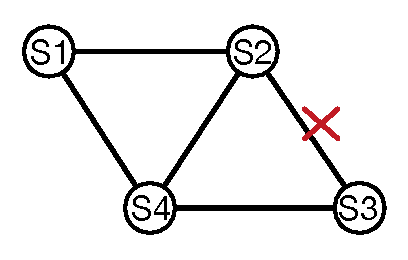
\includegraphics[width=0.3\textwidth] {figs/reconfiguration_a}
	}
	\subfloat[short for lof][Routing spanning tree \textbf{T1}.]{
		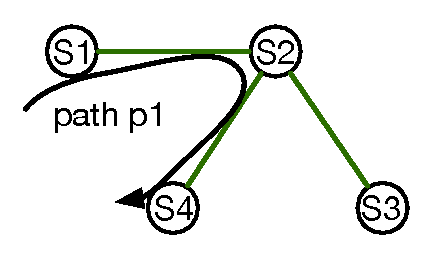
\includegraphics[width=0.25\textwidth] {figs/reconfiguration_b}
	}
	\subfloat[short for lof][Routing spanning tree \textbf{T2}.]{
		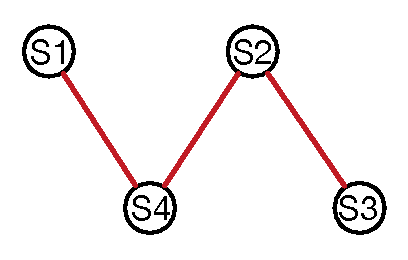
\includegraphics[width=0.25\textwidth] {figs/reconfiguration_c}
	}
	
	\subfloat[short for lof][Three deadlock-free reconfiguration schmes.] {
		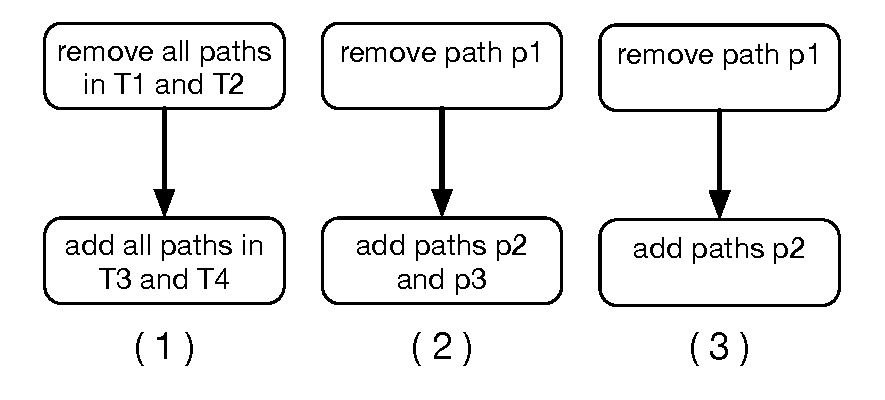
\includegraphics[width=0.4\textwidth] {figs/reconfiguration_f}
	}
	\subfloat[short for lof][Routing spanning tree \textbf{T3}.] {
		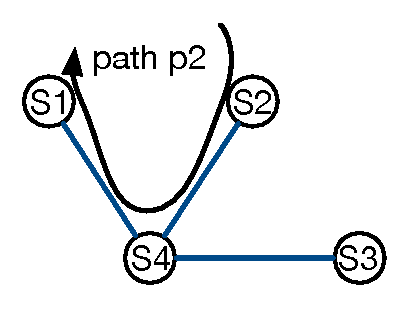
\includegraphics[width=0.25\textwidth] {figs/reconfiguration_d}
	}
	\subfloat[short for lof][Routing spanning tree \textbf{T4}.] {
		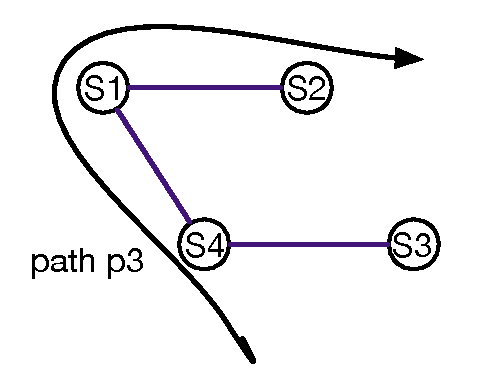
\includegraphics[width=0.25\textwidth] {figs/reconfiguration_e}
	}
	
	\caption{Reconfiguration-induced deadlock case.}\label{fig:reconfigdeadlock}
	
\end{figure*}

In this part, we use an example to show 1) cyclic buffer dependency can be generated if the routing reconfiguration is not well planed; 2) a bad deadlock-free reconfiguration plan will lead to a slow reconfiguration process.

As shown in Fig.~\ref{fig:reconfigdeadlock}(a), in this example we consider a 4-node network \textbf{N}. Fig.~\ref{fig:reconfigdeadlock}(b)-(c),(e)-(f) are four spanning trees \textbf{T1}-\textbf{T4} which specify the routing paths that can be used in \textbf{N}. For example, path p1 is a legal routing path specified in T1.  

Let $\textbf{R}_i$ be the set of paths specified in tree \textbf{Ti}. Let $\textbf{R}_s = \textbf{R}_1 \cup \textbf{R}_2$, and $\textbf{R}_t = \textbf{R}_3 \cup \textbf{R}_4$. It is easy to check both $\textbf{R}_s$ and $\textbf{R}_t$ are deadlock-free routing functions. Initially,  $\textbf{R}_s$ are used as the routing function of \textbf{N}. Due to the failure of link S2-S3, switch S3 becomes unreachable. To maintain the connectivity of \textbf{N}, we can perform a routing reconfiguration to transition from $\textbf{R}_s$ to $\textbf{R}_t$.

During the reconfiguration process, if path p2 in \textbf{T3} and path p3 in \textbf{T4} are added to the routing function before path p1 in \textbf{T1} is removed, a cyclic buffer dependency will be generated. This may cause a PFC deadlock as we explained in Sec.~\ref{subsec:pfcdeadlock}.

In Fig.~\ref{fig:reconfigdeadlock}(d), we present three possible deadlock-free reconfiguration schmes. The first scheme is to remove all the paths in \textbf{T1} and \textbf{T2} before adding any new paths in \textbf{T3} and \textbf{T4}. This scheme will lead to a slow reconfiguration process as all the operations of adding new paths are delayed by the operations of removing old paths. 

The second scheme only requires path p1 is removed before paths p2 and p3 are added. All the other paths not mentioned can be updated freely without any order constraint. Hence the speed of routing reconfiguration can be improved. The third scheme is an optimized reconfiguration scheme in terms of imposing minimum order constraints on the update actions. The intuition here is that as long as paths p1, p2 and p3 do not take effect at the same, deadlock-free can be well guaranteed. 

While for this example it may seem easy to find a deadlock-free reconfiguration scheme that requires minimum order constraints, in general it is difficult as there are combinatorial such schemes to be checked.


\subsection{Measurement of Rule Update Time}\label{subsec:updatetime}

In this part, we demonstrate that adding order constraints to the update of switch rules will significantly prolong the reconfiguration process.
